\documentclass[12pt,a4paper]{article}

\usepackage[utf8]{inputenc}
\usepackage{graphicx}
\usepackage{amsmath}
\usepackage{amssymb}
\usepackage[hidelinks]{hyperref}
\usepackage{geometry}
\usepackage{float}
\usepackage{caption}
\usepackage{subcaption}

\geometry{
    left=25mm,
    right=25mm,
    top=25mm,
    bottom=25mm
}

% Title Page Information
\title{\textbf{MMI712 Project Phase 1 Report}}
\author{Okan Berhoglu}
\date{\today}

\begin{document}

% Title Page
\maketitle
\thispagestyle{empty}
\newpage

\tableofcontents
\newpage

\begin{abstract}
    \textit{This report describes the implementation of a Visual Question Answering (VQA) system using the Moondream model. The application is containerized with Docker to ensure easy deployment and reproducibility. A command-line interface (CLI) allows users to ask questions about images. The project demonstrates how to run efficient vision-language models on local hardware.}
\end{abstract}

\section{Introduction}
Recent advancements in Artificial Intelligence have led to the development of powerful Vision Language Models (VLMs) capable of understanding and generating text based on visual inputs. Models such as GPT-4V and Gemini have demonstrated remarkable capabilities in tasks ranging from image captioning to complex visual reasoning. Despite their performance, these state-of-the-art models often present significant challenges for practical deployment. Many are proprietary, limiting accessibility and research transparency. Furthermore, their substantial computational requirements make them unsuitable for resource-constrained environments, such as edge devices or local applications where latency and privacy are critical concerns. This necessitates the exploration of efficient, open-source alternatives that balance performance with resource utilization.

Moondream emerges as a compelling solution in this landscape. It is a small, open-source vision language model designed to run efficiently on consumer-grade hardware and even mobile devices. By leveraging a compact architecture, Moondream significantly reduces the computational overhead associated with traditional VLMs without sacrificing essential capabilities. Consequently, Moondream offers a practical pathway for deploying visual understanding capabilities in real-world scenarios where resource efficiency and accessibility are paramount. 

To ensure reproducibility and streamline the deployment process, Docker is utilized to containerize the application. Docker provides a lightweight and portable environment that encapsulates the application and its dependencies, eliminating the "it works on my machine" problem. By defining the runtime environment in a Dockerfile, we ensure that the model behaves consistently across different computing platforms. This approach simplifies the setup process for other researchers and developers, allowing them to easily deploy and experiment with software applications or models without worrying about conflicting libraries or system configurations.

In this work, the Moondream model is implemented for Visual Question Answering (VQA) tasks. The model processes natural language questions about input images and generates corresponding natural language answers. To ensure consistency and ease of deployment, the application is containerized using Docker. The implementation is validated using a set of test images and questions, and users interact with the application through a Command Line Interface (CLI).

This report is structured as follows; after the introduction, the methodology section describes the technical details of the implementation, an example usage of the docker image is given in the results section and the usage of the application is given in the usage section. Lastly the conclusion section provides a summary of the work done.

\section{Methodology}
The moondream model is implemented for Visual Question Answering (VQA) tasks. The model processes natural language questions about input images and generates corresponding natural language answers. To ensure consistency and ease of deployment, the application is containerized using Docker. A docker image is created and pushed to Docker Hub. The docker image is then used to run the application. The docker image contains the moondream model, the application code, and the required dependencies.

The phase of the project contains a docker file, a requirements file and two python scripts. One of the scripts is used to install the model and the other one is the main script which the user interacts with.

The main script which is the "main.py" file, serves as the entry point for the application. It requires the path to an input image. Upon execution, the script loads the Moondream model. The specified image is then loaded and encoded by the model. The script enters an interactive loop where it waits for the user to input questions about the image. These questions are processed by the model, which generates and displays the corresponding answers. The loop continues until the user interrupts the process (e.g., via CTRL+C), ensuring a continuous and interactive user experience.

The other script which is the "model\_installer.py" file, is used to install the Moondream model. Upon execution, the script downloads the Moondream model from the Hugging Face model hub and saves it to the local machine using the "snapshot\_download" function from the "huggingface\_hub" library.

To facilitate the deployment, a Dockerfile is provided. This file defines the environment for the application. It starts with a lightweight Python 3.10 slim image. It then installs necessary system dependencies like git. The project files, including the requirements and scripts, are copied into the container. The Python dependencies listed in requirements file are installed. Crucially, the "model\_installer.py" script is executed during the build process to pre-download the Moondream model, ensuring it is baked into the image. Finally, the entry point is set to run the main application script.

\section{Usage}
\label{sec:usage}
The resulting image is published in the docker hub. The application can be found in this link:
\url{https://hub.docker.com/r/okanberhoglu/mmi712_project_moondream}

After downloading the image, the application can be run using the following command:
{\fontsize{7pt}{7pt}\selectfont
\begin{verbatim}
docker run -it --rm -v <path_to_image_folder>:/data:ro okanberhoglu/mmi712_project_moondream:latest --image_path /data/<image_name>
\end{verbatim}
}

The given command runs the Docker image in interactive mode and removes the container automatically after it exits, ensuring that no temporary containers remain on the system. The "\texttt{-v <path\_to\_image\_folder>:/data:ro}" option mounts a local directory containing the input image into the container at the "/data" path in read-only mode, allowing the container to access the image without modifying the host files. The Docker image "okanberhoglu/mmi712\_project\_moondream:latest" encapsulates all required dependencies and the inference environment. The "\texttt{--image\_path /data/<image\_name>}" argument is passed directly to the application inside the container and specifies the exact location of the input image to be processed.

\section{Results}
An example usage of the application and the results are given in this section. Firstly the test input image is given in the figure \ref{fig:test}.

\begin{figure}[H]
    \centering
    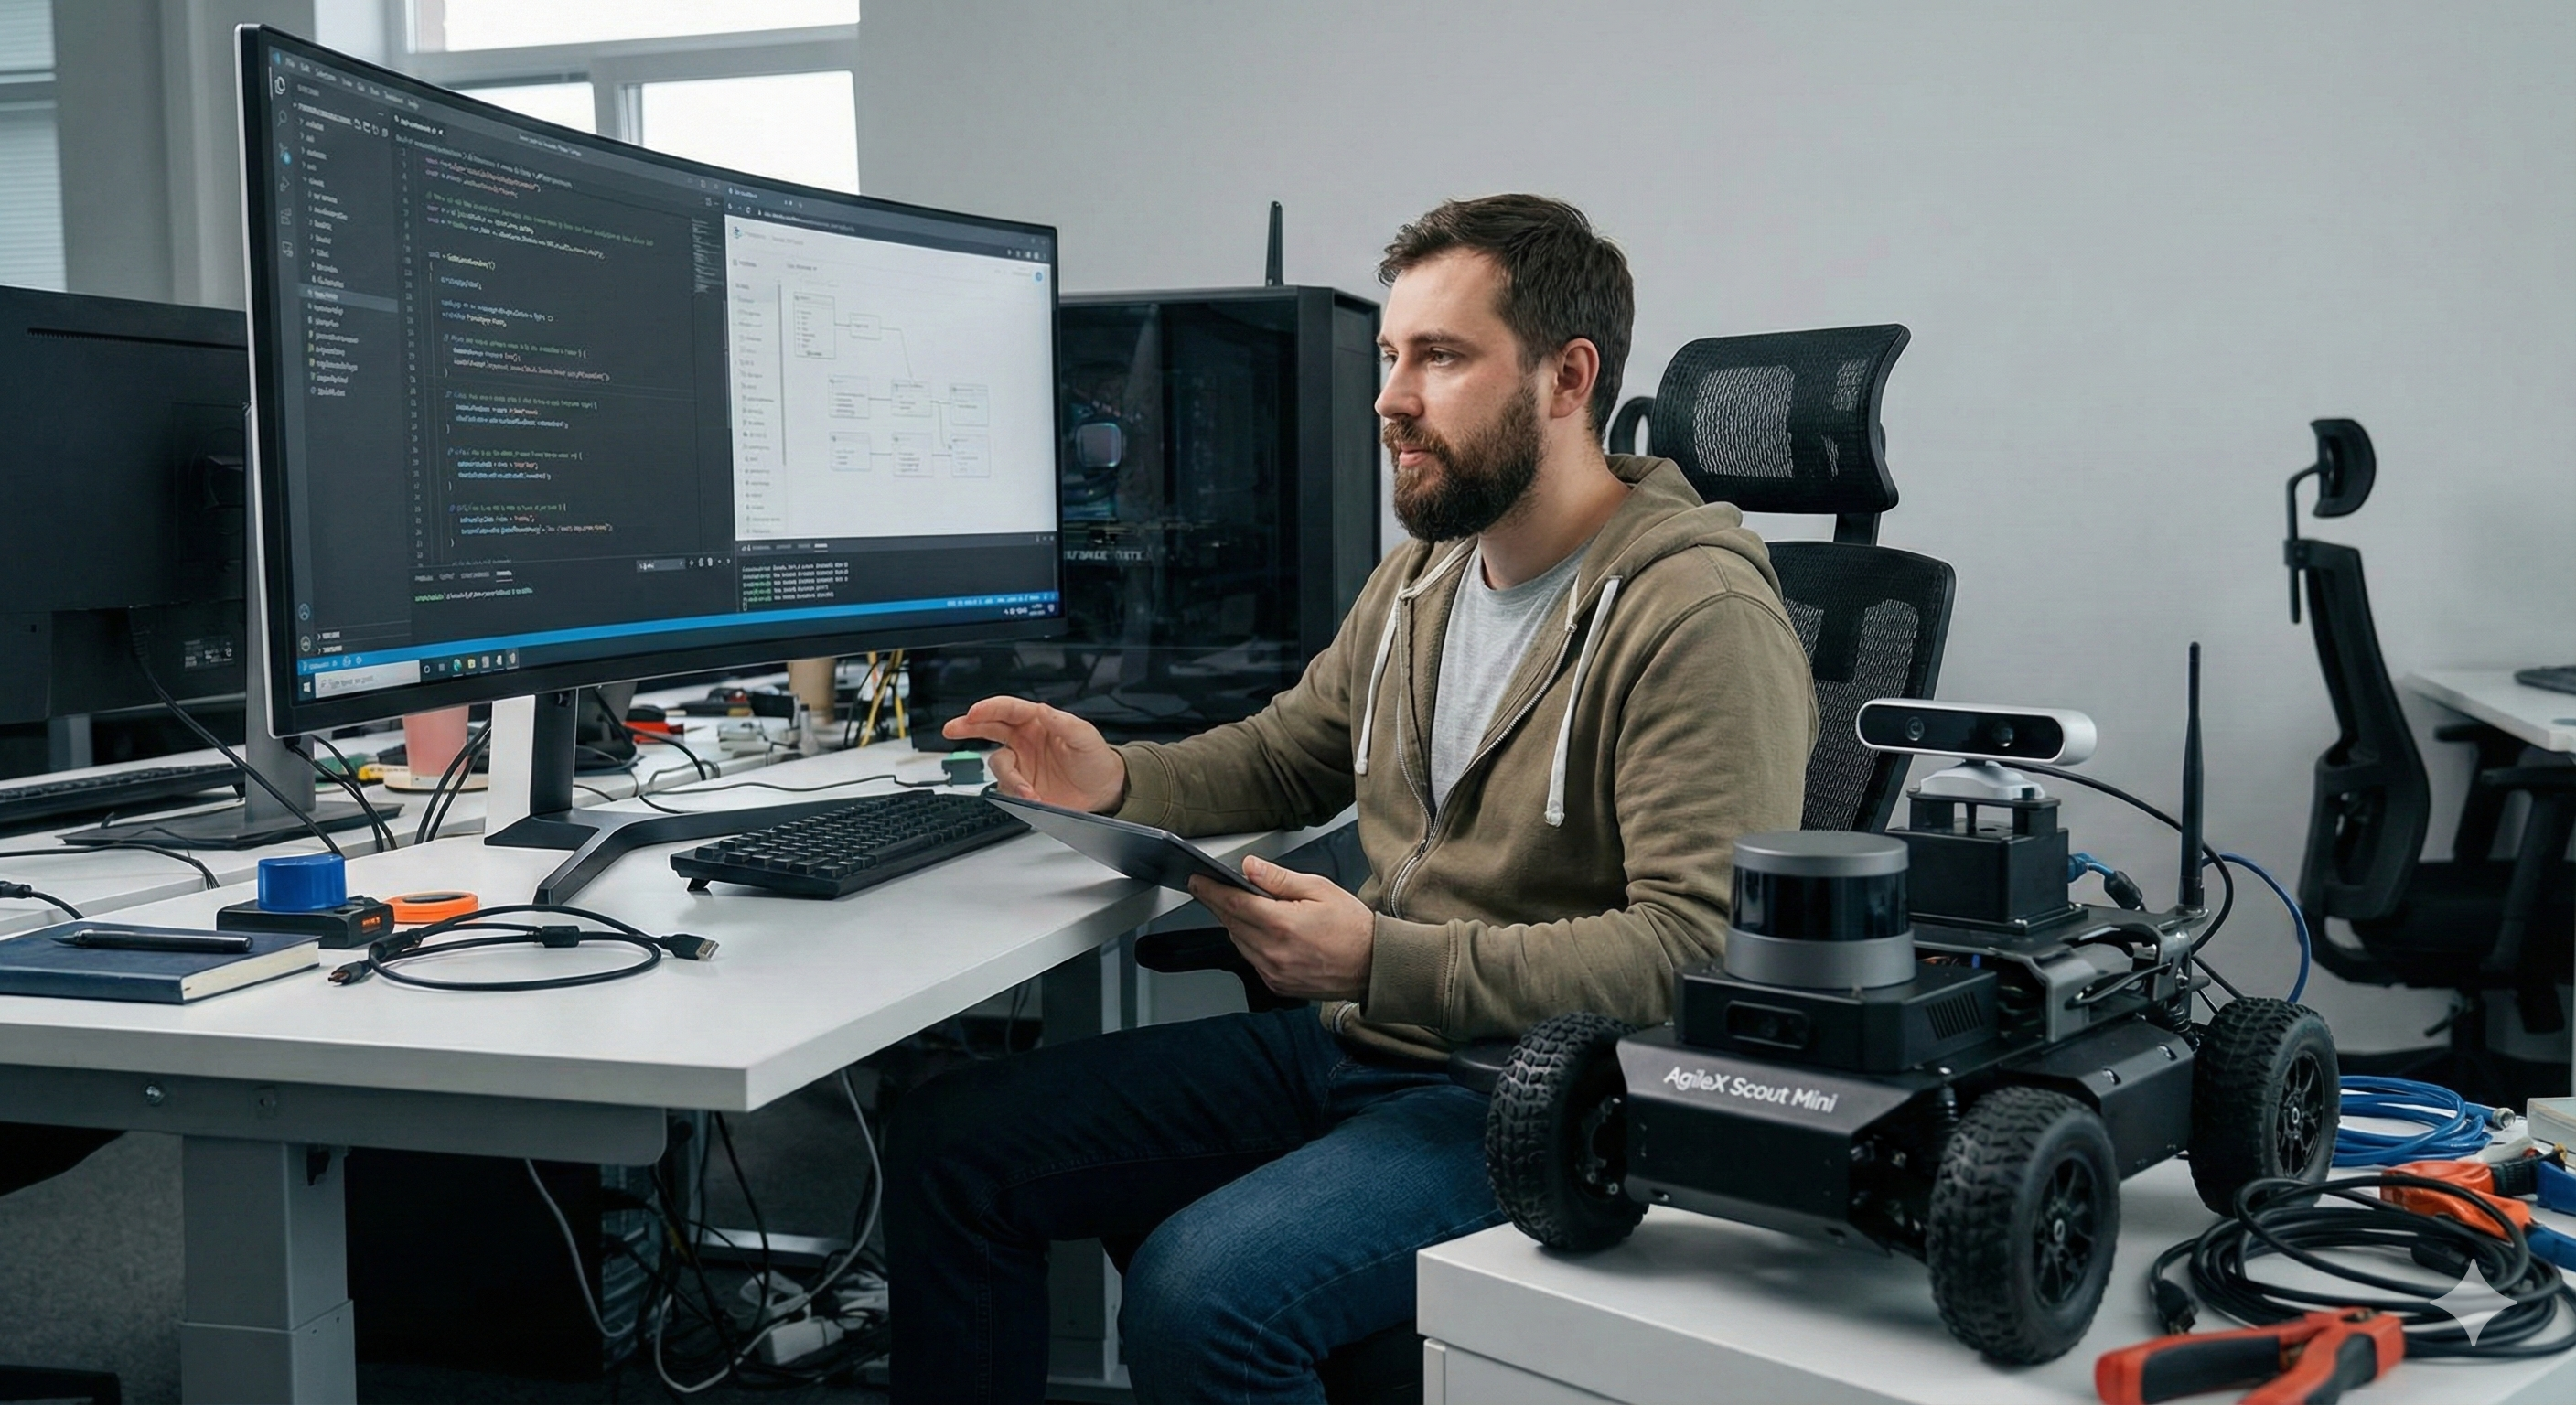
\includegraphics[width=350pt]{test_image.png}
    \caption{Example input image.}
    \label{fig:test}
\end{figure}
After running the application with the command given in the section \ref{sec:usage}, the application can be used as shown in the figures \ref{fig:q1} and \ref{fig:q2}.

\begin{figure}[H]
    \centering
    \includegraphics[width=400pt]{q1.png}
    \caption{Example usage.}
    \label{fig:q1}
\end{figure}
\begin{figure}[H]
    \centering
    \includegraphics[width=350pt]{q2.png}
    \caption{Example usage with questions.}
    \label{fig:q2}
\end{figure}

\section{Conclusion}
In this project, the Moondream vision language model was successfully containerized using Docker. A Dockerfile was created to automate the installation of dependencies and the model itself, ensuring a consistent and reproducible environment. A Python script was developed to interface with the model, allowing users to perform Visual Question Answering tasks via a command-line interface. This implementation simplifies the deployment process and demonstrates the feasibility of running efficient VLMs on local hardware.

\begin{thebibliography}{9}

\bibitem{moondream}
Moondream.ai. \textit{Moondream: A tiny vision language model}. Available at: \url{https://moondream.ai/} (Accessed: \today).

\bibitem{huggingface}
Hugging Face. \textit{Hugging Face: The AI community building the future}. Available at: \url{https://huggingface.co/} (Accessed: \today).

\bibitem{docker}
Docker. \textit{Docker Documentation}. Available at: \url{https://docs.docker.com/} (Accessed: \today).

\end{thebibliography}

\end{document}
